% Created 2013-12-20 金 04:52
\documentclass[12pt]{jsarticle}
\usepackage[dvipdfmx]{graphicx}
\usepackage{comment}
%%\date{\today}
%\title{}
\textheight = 25truecm
\textwidth = 18truecm
\topmargin = -1.5truecm
\oddsidemargin = -1truecm
\evensidemargin = -1truecm
\marginparwidth = -1truecm
\def\theenumii{\Alph{enumii}}
\def\theenumiii{\alph{enumiii}}
\def\labelenumi{(\theenumi)}
\def\labelenumiii{(\theenumiii)}
\begin{document}

%\maketitle
%\tableofcontents

\begin{center}
%%%%%%%%%%%%%%%%%%%%%%%%%%%%%%%%%%%%%%%
%%%タイトル                         %%%
%%%%%%%%%%%%%%%%%%%%%%%%%%%%%%%%%%%%%%%
{\LARGE 「Mintオペレーティングシステムを用いた割り込み処理のデバッグ支援環境の提案」の要約}
\end{center}

\begin{flushright}
  2014/5/19\\
  藤田将輝
\end{flushright}
%%%%%%%%%%%%%%%%%%1章%%%%%%%%%%%%%%%%%%%
\section{はじめに}
本資料では山本の特別研究報告書の概要を理解し,整理するため,山本の特別研究報告書である
「Mintオペレーティングシステムを用いた割り込み処理のデバッグ支援環境の提案」\cite{yama}
の要約を示す.

%%%%%%%%%%%%%%%%%%2章%%%%%%%%%%%%%%%%%%%
\section{仮想計算機を用いたOSデバッグ手法}




\begin{comment}
\subsection{構成}
仮想計算機方式にはベアメタル型とホストOS型の2種類ある.
以下でその概要について示す.
\begin{enumerate}
\item ベアメタル型

ベアメタル型ではハードウェア上でハイパーバイザが走行し,ハイパーバイザ上で
デバッグ支援OSとデバッグ対象OSが走行する.
\item ホストOS型

ホストOS型ではハードウェア上でホストOSが走行し,ホストOS上でデバッグ支援アプリケーション
とハイパーバイザが走行する.また,ハイパーバイザ上でデバッグ対象OSが走行する.
\end{enumerate}
\end{comment}



\subsection{デバッグ手法の概要}
仮想計算機を用いたOSデバッグ手法で,割り込み処理のデバッグが可能な手法として
割り込み挿入手法とロギング/リプレイ手法がある.
以下にその概要を示す.
\begin{enumerate}
\item 割り込み挿入手法

割り込み挿入手法では,プログラマがデバッグ対象OSのコードにハイパーコールを挿入する.
デバッグ対象OSの走行時,ハイパーコールを挿入したコード位置に単一の割り込みを発生させ,
割り込みを再現することで,デバッグを支援する.


\item ロギング/リプレイ手法

ロギング/リプレイ手法ではロギングとリプレイにより,割り込み処理を含めたバグ発生時点までの処理の流れを
再現することで,デバッグを効率化する.
ロギングとはデバッグ対象の処理の流れを保存することで,リプレイとはロギングで保存した情報から
処理の流れを再現することである.

\end{enumerate}
\begin{comment}
\subsection{割り込み挿入手法における処理流れ}
割り込み挿入手法における処理流れを以下に示す.Virtual Machine Control Structure(以下,VMCS)
はハイパーバイザが仮想計算機の走行状態を変更するためのデータ構造体である.これの変更により,
仮想計算機に割り込みを発生することができる.
\begin{enumerate}
\item 割り込み発生要求

ハイパーコールにより,デバッグ対象OSがハイパーバイザのデバッグ支援機構へ割り込みを行う.
\item データ生成要求

ハイパーバイザのデバッグ支援機構がデバッグ支援OSのデバッグ支援機構に対し,割り込み処理で使用するデータを生成要求する.
\item データの生成

割り込み処理で使用するデータをデバッグ支援OSからのデバッグ支援機構が生成する.
\item データ生成完了通知

デバッグ支援OSの支援機構からハイパーバイザのデバッグ支援機構へデータ生成完了を通知する.
\item VMCSの変更

ハイパーバイザがVMCSを変更する.
\item 割り込み発生

ハイパーバイザから仮想計算機へ処理が遷移する.その後,デバッグ対象OSへ単一の割り込みが発生する.
\end{enumerate}
\subsection{ロギング/リプレイ手法における処理流れ}
\subsubsection{ロギングの処理流れ}
ロギングの例としてベアメタル型を用いたロギング/リプレイ手法における
ロギングの処理流れについて以下に示す.
\begin{enumerate}
\item 割り込み発生

デバッグ対象OSで割り込みが発生し,デバッグ対象OSの処理が中断される.その後,ハイパーバイザの支援機構へ処理が遷移する.
\item 再現情報の格納

ハイパーバイザの支援機構が再現情報をメモリへ格納する
\item 割り込み処理の開始

デバッグ対象OSへ処理が遷移し,デバッグ対象OSが割り込み処理を開始する.
\end{enumerate}
\subsubsection{リプレイの処理流れ}
リプレイの例としてベアメタル型を用いたロギング/リプレイ手法における
リプレイの処理流れについて以下に示す.
\begin{enumerate}
\item 再現情報の取得

ハイパーバイザの支援機構がロギング時に保存した再現情報をメモリから取得する.
\item 割り込み発生アドレスまでの処理の実行

デバッグ対象OSが再現情報の割り込み発生アドレスまで処理を実行する.
\item 分岐回数の比較

ハイパーバイザの支援機構が再現情報の分岐回数と現在の分岐回数を比較する.
\item 割り込みの発生

デバッグ対象OSへ割り込みが発生する.
\end{enumerate}
\end{comment}
\subsection{問題点}
仮想計算機を用いたデバッグ手法の問題点を以下に示す.
\begin{enumerate}

\item 実計算機で発生する間隔での複数の割り込みが困難

割り込み挿入法ではデバッグ対象OSのコードにハイパーコールを挿入し,
割り込みを発生させるため,コードが実行されるタイミングはOSの処理速度に依存する.
このためCPUへ発生する間隔で複数の割り込み(以下,実割り込み)が発生する間隔を調整することは
困難である.
ロギング/リプレイ手法ではではデバッグ対象OSとハイパーバイザの間の処理の遷移や再現情報の格納による処理
負荷が発生する.このため,実割り込みがロギング中に発生しないと考えられる.ロギング中に実割り込みが
発生しない場合,実割り込みを再現するための再現情報を保存できない.このため,実割り込みの発生が困難である.


\item 任意のタイミングでの割り込み発生が困難

ロギングリプレイ手法において,任意のタイミングで割り込みを発生させるためには,再現情報として
割り込みを発生させるアドレスと分岐回数をプログラマが用意しなければならない.
これらの指定が困難であるため,任意のタイミングで割り込みを発生させることが困難である

\begin{comment}
\item 実割り込みの発生が困難

ロギングにおけるデバッグ対象OSとハイパーバイザの間の処理の遷移や再現情報の格納による処理
負荷が発生する.このため,実割り込みがロギング中に発生しないと考えられる.ロギング中に実割り込みが
発生しない場合,実割り込みを再現するための再現情報を保存できない.このため,実割り込みの発生が困難である.
\end{comment}

\end{enumerate}

%%%%%%%%%%%%%%%%%%3章%%%%%%%%%%%%%%%%%%%
\section{Mintオペレーティングシステム}
\subsection{Mintの設計方針}
Mintは1台の計算機上で複数のLinuxを独立に走行させる方式である.
Mintの設計方針として,以下の2つがある.
\begin{enumerate}
\item すべてのLinuxが相互に処理負荷の影響を与えない.
\item すべてのLinuxが入出力性能を十分に利用できる.
\end{enumerate}
\subsection{Mintの構成}
Mintでは,1台の計算機上でCPU,メモリ,およびデバイスを分割し,各OSが占有する.
Mintの構成例を以下で説明する.
\begin{enumerate}
\item CPU

コア単位で分割し,各OSノードがコアを1つ以上占有する
\item メモリ

空間分割し,各OSノードが分割領域を占有する.
\item デバイス

デバイス単位で分割し,各OSノードが指定されたデバイスを占有する.
\end{enumerate}
%%%%%%%%%%%%%%%%%%4章%%%%%%%%%%%%%%%%%%%
\section{設計}
\subsection{設計の目的}
Mintを用いた割り込み処理のデバッグ支援環境を設計する目的について以下に示す.
\begin{enumerate}

\item 実割り込みを発生させる環境の提供

割り込みの発生感覚に依存するバグを確認するためには,実割り込みを発生させる必要がある.
しかし,仮想化を用いたデバッグ手法で実割り込みを発生させることは困難である.
そこでMintを用いた割り込み処理のデバッグ支援環境では,デバッグ対象OSへ実割り込みを発生させる環境を提供する.
\item 任意のタイミングで割り込みを発生させる環境の提供

デバッグの際,デバッグ対象処理のバグの有無やバグの発生個所を確認するために,デバッグ対象の処理を繰り返し
実行する.しかし割り込み処理は割り込みが非同期的に発生するため,繰り返し実行することが困難である.
また,仮想計算機を用いたデバッグ手法では,任意のタイミングで割り込みを発生させることが困難である.
Mintを用いた割り込み処理のデバッグ支援環境では,任意のタイミングで割り込みを発生できる環境を提供する.
\end{enumerate}
\subsection{設計における課題}
Mintを用いた割り込み処理のデバッグ支援環境における課題について以下に示す.
\begin{enumerate}
\item ハイパーバイザを用いないデバッグ支援環境の提供

実割り込みを発生させる環境を実現するため,ハイパーバイザによる処理負荷のない環境が必要となる.
このため,ハイパーバイザを用いないデバッグ支援環境を提供する.
\item デバッグ対象OSがデバッグ支援機構の処理負荷の影響を受けないデバッグ支援環境の提供

デバッグ対象OSがデバッグ支援機構の処理機構の処理負荷を受けると,実割り込みが発生しない.
このため,デバッグ対象OSがデバッグ支援機構の処理負荷の影響を受けないデバッグ支援環境を提供する
\item CPUへの実割り込みの発生

割り込み挿入手法のようにデバッグ対象OSのコードにハイパーコールを挿入して割り込みを発生させると,実割り込みの
発生が困難である.
実割り込みを発生させる環境を実現するため,デバッグ対象OSのCPUへ割り込みを発生させる.

\end{enumerate}
\subsection{設計における課題への対処}
Mintを用いた割り込み処理のデバッグ支援環境における課題への対処を以下に示す.
\begin{enumerate}
\item Mintを用いたデバッグ対象OSとデバッグ支援OSの同時走行

課題(1)と(2)への対処としてMintを用いてデバッグ対象OSとデバッグ支援OSを同時走行させる.
Mintは仮想化によらず複数OSを同時走行させるため,ハイパーバイザのよる
処理負荷が発生しない.また,デバッグ対象OSがデバッグ支援OSの影響を受けないため,デバッグ対象OS
がデバッグ支援機構の影響を受けない.
\item Inter-Processor Interruptの送信

課題(3)への対処として,Inter-Processor Interrupt(以下,IPI)を利用する.
実際にCPUへ割り込みを発生させるため,実割り込みや任意のタイミングでの割り込みを発生させられる.
\end{enumerate}
\subsection{Mintを用いた割り込み処理のデバッグ支援環境の構成}

\begin{figure}[t]
\begin{center}
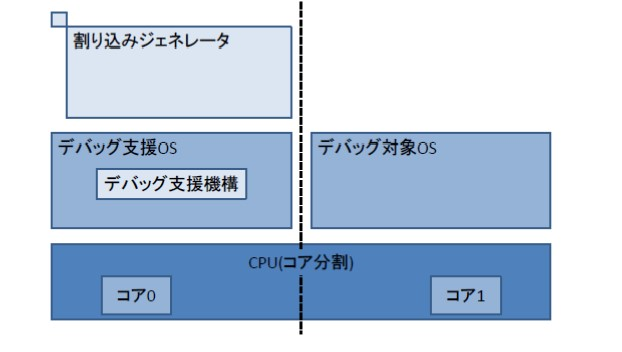
\includegraphics[height=7.0cm]{./fig2.jpg}          
\caption{Mintを用いた割り込み処理のデバッグ支援環境の構成}
\label{fig:2}
\end{center}
\end{figure}



Mintを用いた割り込み処理のデバッグ支援環境の構成例を図1に示す.
このデバッグ支援環境では,ハードウェア上でデバッグ対象OSとデバッグ支援OSが走行する.
また,デバッグ支援OSにデバッグ支援機構を実装し,この機構を利用する割り込みジェネレータをアプリケーションとして
実装する.
割り込みジェネレータ,デバッグ支援機構,デバッグ支援OS,およびデバッグ対象OSについて,以下で説明する.
\begin{enumerate}
\item 割り込みジェネレータ

プログラマが割り込み情報を指定する際に利用するアプリケーションである.

\item デバッグ支援機構

割り込みジェネレータから通知される割り込み情報をもとに,デバッグ対象OSへIPIを送信する機構である.
\item デバッグ支援OS

デバッグ支援機構を実装して,走行しているOSである.
\item デバッグ対象OS

デバッグの対象となるOSである.
\end{enumerate}
\subsection{Mintを用いた割り込み処理のデバッグ支援環境における処理流れ}


\begin{figure}[t]
\begin{center}
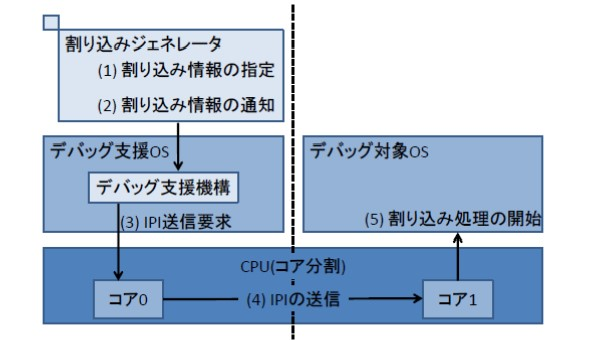
\includegraphics[height=7.0cm]{./fig1.jpg}          
\caption{Mintを用いた割り込み処理のデバッグ支援環境におけるデバッグ処理の流れ}
\label{fig:up}
\end{center}
\end{figure}




Mintを用いた割り込み処理のデバッグ支援環境における処理流れを図2に示し以下で説明する.
\begin{enumerate}
\item 割り込み情報の指定

プログラマが割り込みジェネレータを用いて割り込み情報を指定する
\item 割り込み情報の通知

割り込みジェネレータからデバッグ支援OSのデバッグ支援機構へ割り込み情報を通知する.
\item IPI送信要求

割り込み情報をもとに,デバッグ支援OSのデバッグ支援機構からコア0へIPI送信要求を行う.
\item IPIの送信

コア0からコア1へ送信する.
\item 割り込み処理の開始

デバッグ対象OSが割り込み処理を開始する.
\end{enumerate}
%%%%%%%%%%%%%%%%%%5章%%%%%%%%%%%%%%%%%%%
\section{実装}
\subsection{実装例}
デバイスの1つであるNICのパケット受信割り込みを発生させる環境を実現する.
これにより,Mintにおける割り込み処理のデバッグ支援環境で,割り込み処理が再現できることを示す.
実装例として,NICがパケット受信時に発生させる割り込み(パケット受信割り込み)に対するNICドライバ
の割り込み処理のデバッグ支援環境を実装する.




\begin{comment}
\subsection{NICのパケット受信割り込みの処理流れ}
NICによるパケットの格納と割り込み発生について以下で説明する.
受信バッファはNICが受信したパケットを格納するメモリ領域である.
また,受信ディスクリプタは受信バッファへのアドレスと受信バッファがパケットを受信済みか否かを
示す状態(以下,受信バッファ状態)を保持するメモリ領域である.
\begin{enumerate}
\item 受信バッファアドレスの取得

NICが受信ディスクリプタから受信バッファアドレスを取得する.

\item 受信バッファへのパケットの格納

NICが受信バッファアドレスをもとに,受信バッファへパケットを格納する
\item 受信バッファ状態の更新

NICが受信バッファ状態を受信済み状態に更新する
\item パケット受信割り込みの発生

NICがデバイスドライバへパケット受信割り込みを発生させる.これにより,OSが割り込み処理を開始する.
\item 受信バッファの特定

NICドライバが受信バッファ状態を確認する.これにより,パケットが格納されている受信バッファを特定する.
\item ソケットバッファへのパケットの格納

NICドライバが受信バッファからパケットを取得し,ソケットバッファへ格納する.
\end{enumerate}
\subsection{IPI送信の流れ}
デバッグ対象OSへの割り込み発生方式として,デバッグ対象OSからデバッグ支援OSへのIPIの送信について考える.
MintにおけるIPIの送信の流れとして,OSノード0からOSノード1へIPIを送信する流れについて以下で説明する.
ここで,OSノード0がコア0,OSノード1がコア1を分割占有し走行するものとする.
各コアはLocal Advanced Programmable Interrupt Controller(以下,LAPIC)を保持する.
LAPICはプロセッサの各コアに内蔵される割り込みコントローラである.各LAPICは識別子としてLAPIC IDを持つ.
また,LAPICはInterrupt Command Register(以下,ICR)を保持する.ICRはIPIの送信に用いられるレジスタである.
\begin{enumerate}
\item ICRへの書き込み

コア0が自身のLAPIC中のICRへLAPIC IDと割り込みベクタ番号を書き込む.
なお,割り込みベクタ番号とは割り込みの要因を示す番号である.
\item IPIの送信

ICRへ書き込んだLAPIC IDをもとに,コア0のLAPICからコア1のLAPICへIPIを送信する.
\item 割り込み処理の開始

IPIを受信したコア1のLAPICがOSノード1へ割り込みを発生させる.これにより,OSノード1が割り込み処理を開始する.
この際,OSノード1が割り込みベクタ番号に対応した割り込みハンドラを実行する.
\end{enumerate}
\end{comment}







\subsection{実装における課題}
NICドライバの割り込み処理を対象としたデバッグ支援環境の実装における課題を以下に示す.
\begin{enumerate}
\item NICなしでNICドライバを利用できる環境の提供

NICがパケット受信割り込みや,パケット格納が行われない環境でNICドライバの割り込み処理を確認する必要がある.
ただし,本研究では考察しない.
\item 受信バッファへのパケット格納

パケット割り込み発生後,NICドライバは受信バッファからパケットを取得し,取得したパケットを用いて割り込み処理を行う.
このため,NICの代わりに受信バッファへパケットを格納する.
\item 受信バッファ状態の更新

NICの代わりに受信ディスクリプタの受信バッファ状態を更新する.
\item パケット受信割り込みの発生

NICの代わりにNICドライバへパケット受信割り込みを発生させる.
\item パケット受信割り込みの発生間隔の調整

連続して発生するパケット受信割り込みに対する割り込み処理を確認する際,
パケット受信割り込みの発生間隔を調整する必要がある.ただし,本研究では考察しない.
\end{enumerate}
\subsection{実装における課題への対処}
課題(2)(3)(4)の対処を以下に示す.
\begin{enumerate}
\item デバッグ支援OSによるパケット生成と格納

課題(2)への対処として,デバッグ支援OSがパケットを生成し,格納する.
\item 受信バッファ状態の更新

課題(3)への対処として,デバッグ支援OSが受信ディスクリプタの受信バッファ状態を更新する.
\item デバッグ支援OSによるIPIの送信

課題(3)への対処として,デバッグ支援OSからデバッグ対象OSへのIPIの送信によりパケット受信割り込みを発生させる.
\end{enumerate}
\subsection{NICドライバの割り込み処理を対象としたデバッグ支援環境の構成}
パケット受信割り込みに対するNICドライバの割り込み処理を対象としたデバッグ支援環境の構成例について図3に示し,以下で説明する.


\begin{figure}[t]
\begin{center}
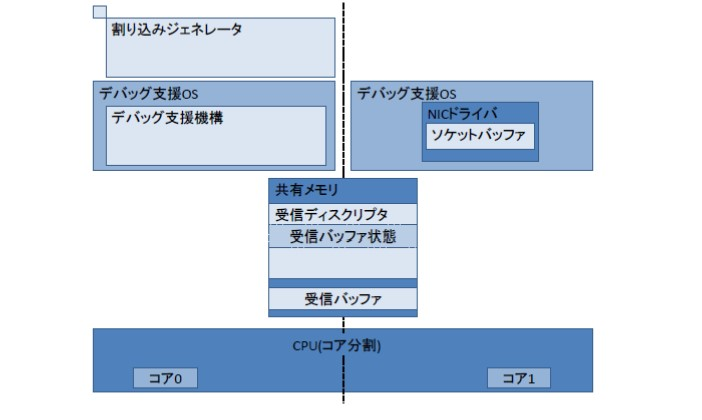
\includegraphics[height=7.0cm]{./fig3.jpg}          
\caption{NICドライバの割り込み処理を対象としたデバッグ支援環境の構成}
\label{fig:up}
\end{center}
\end{figure}



\begin{enumerate}
\item 割り込みジェネレータ

プログラマが割り込み情報を指定する際に用いるアプリケーションである.
\item デバッグ支援OS

デバッグ支援機構を実装し,走行するLinuxである.
\item デバッグ対象OS

Mintを用いて走行するための改変を加えたLinuxである.
\item デバッグ支援機構

デバッグ支援機構のシステムコールである.デバッグ支援機構として以下の機能を持つ.
\begin{enumerate}
\item パケットの生成
\item パケットの格納
\item 受信バッファ状態の更新
\item 割り込み情報をもとにしたIPIの送信
\end{enumerate}
\item NICドライバ

デバッグ対象OSの保持するNICドライバである.
\end{enumerate}
\subsection{NICドライバの割り込み処理を対象としたデバッグ支援環境における処理流れ}
NICドライバの割り込み処理を対象としたデバッグ支援環境における処理流れについて図4に示し,以下で説明する.


\begin{figure}[t]
\begin{center}
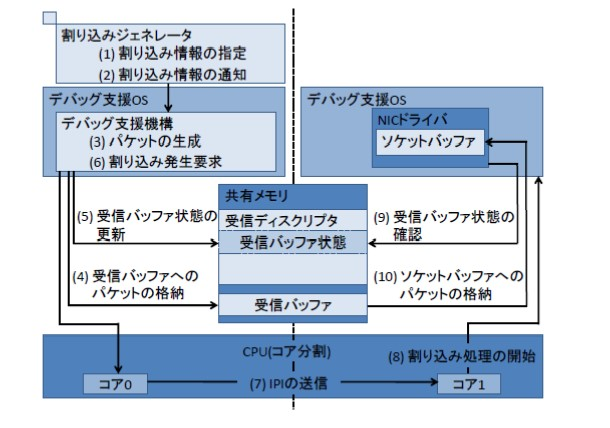
\includegraphics[height=7.0cm]{./fig4.jpg}          
\caption{NICドライバの割り込み処理を対象としたデバッグ支援環境における処理流れ}
\label{fig:up}
\end{center}
\end{figure}


\begin{enumerate}
\item 割り込み情報の指定

プログラマが割り込みジェネレータを用いて割り込み情報を指定する.
\item 割り込み情報の通知

割り込みジェネレータからデバッグ支援OSのデバッグ支援機構へ割り込み情報を通知する
\item パケット生成

デバッグ支援OSのデバッグ支援機構がパケットを生成する.
\item 受信バッファへのパケット格納

デバッグ支援OSのデバッグ支援機構が受信バッファへのパケットを格納する
\item 受信バッファ状態の更新

デバッグ支援OSのデバッグ支援機構が受信バッファ状態を受信済み状態へ更新する.
\item 割り込み発生の要求

割り込み情報をもとに,デバッグ支援OSのデバッグ支援機構からコア0へ割り込み発生要求を行う.
\item IPIの送信

デバッグ支援OSが保持するコア0からデバッグ対象OSが保持するコア1へIPIを送信する.
\item 割り込み処理の開始

デバッグ対象OSが割り込み処理を開始する.この際,デバッグ対象OSが割り込みベクタ番号に対応した割り込みハンドラを実行する.
\item 受信バッファの特定

受信ディスクリプタが保持する受信バッファ状態をデバッグ対象OSのNICドライバが参照する.
これにより,パケットが格納されている受信バッファを特定する.
\item ソケットバッファへのパケット格納

受信バッファからソケットバッファへデバッグ対象OSのNICドライバがパケットを格納する
\end{enumerate}
%%%%%%%%%%%%%%終わりに%%%%%%%%%%%%
\section{終わりに}
本資料では論文「Mintオペレーティングシステムを用いた割り込み処理のデバッグ支援環境の提案」
の要約を示した.
従来のデバッグ方法の概要と問題点を確認できた.さらにその問題点をMintを用いて解決する方法を理解できた.
現在,IPIを用いてCPUへ割り込みを発生できた.
NICドライバへの割り込みのデバッグ環境の構成はまだ完成していない.
今後はMintを用いた割り込み処理のデバッグ支援環境を構築するために,
割り込み処理とIPIの送受信について理解を深め,問題の解決に臨む.


\begin{thebibliography}{9}
\bibitem{yama} 山本凌平:Mintオペレーティングシステムを用いた割り込み処理のデバッグ支援環境の提案,
岡山大学工学部情報工学科特別研究報告(2014).
\end{thebibliography}

\end{document}
